\documentclass[assd_tp3_main.tex]{subfiles}

\begin{document}

\section{SAR}

\subsection{Introducci\'on}

El primer conversor que se implement\'o fue un registro de aproximaciones sucesivas, o SAR por sus siglas en ingl\'es (Successive Approximation Register). El diagrama de bloques de este conversor se observa en la figura \ref{fig:sar-bloques}.


\begin{figure}[ht!]
	\centering
	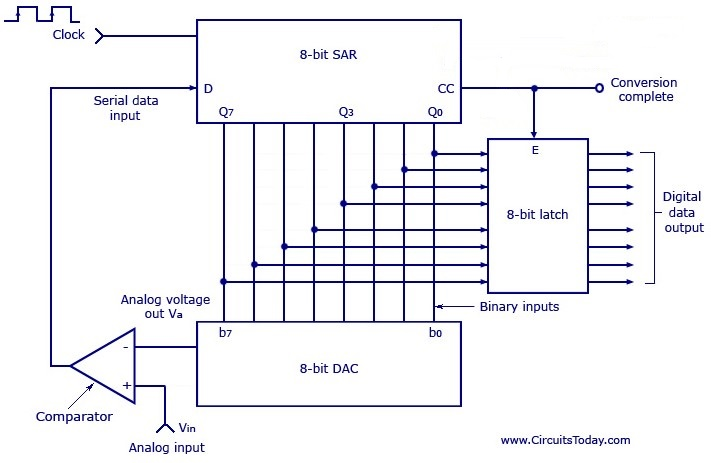
\includegraphics[width=0.8\textwidth]{images/ej2/sar-bloques.jpg}
	\caption{Diagrama en bloques del SAR}
	\label{fig:sar-bloques}
\end{figure}

La l\'ogica de predicci\'on del SAR sigue el principio de la b\'usqueda binaria. Se comienza con el bit m\'as significativo en 1 y el resto en 0, se convierte esta se\~nal al dominio anal\'ogico, y se la compara con la entrada. Seg\'un el resultado de esta comparaci\'on (a la cual se la puede considerar una cuantizaci\'on de un bit), el bit se dejar\'a encendido o se apagar\'a en la siguiente iteraci\'on, en la cual adem\'as se encender\'a el bit siguiente. El proceso se repite sucesivamente hasta llegar al bit menos significativo, luego de lo cual se enciende la se\~nal de end of conversion, guardando el resultado de la conversi\'on en el latch de salida. Como para cada conversi\'on de N bits se deben hacer N+1 comparaciones, entonces se requiere que la frecuencia del clock que controla al registro de aproximaciones sucesivas sea:

\begin{equation}
	f_{CLK} = 9f_s
\end{equation} 

Adicionalmente, es necesario que la se\~nal de entrada se mantenga constante durante el tiempo de conversi\'on, o al menos que vari\'e menos de un LSB. por lo tanto, la misma debe atravesar un sample and hold antes de ingresar al comparador.



\subsection{Implementaci\'on}






\subsection{Mediciones}

\end{document}

